\section{Оглавление}
(Ссылки кликабельны)\\
\hyperlink{p1}{Задание.....................................................................................................................................................3}\\
\hyperlink{p2}{Выполнение...............................................................................................................................................3}\\
\hyperlink{p3}{Исходный код............................................................................................................................................5}\\
\hyperlink{p4}{Вывод........................................................................................................................................................5}\\
\newpage
\section{Задание}

\hypertarget{p1}1 - {Для} указанной функции провести модульное тестирование разложения функции в степенной ряд. Выбрать достаточное тестовое покрытие. \\
2 - Провести модульное тестирование указанного алгоритма. Для этого выбрать характерные точки внутри алгоритма, и для предложенных самостоятельно наборов исходных данных записать последовательность попадания в характерные точки. Сравнить последовательность попадания с эталонной.\\
3 - Сформировать доменную модель для заданного текста. Разработать тестовое покрытие для данной доменной модели

\section{Выполнение}
\subsection{Задание 1:}
\hypertarget{p2}{}
Так как функция определена на отрезке от -1 до 1
достаточным тестовым покрытием будет являться покрытие семи точек.\\
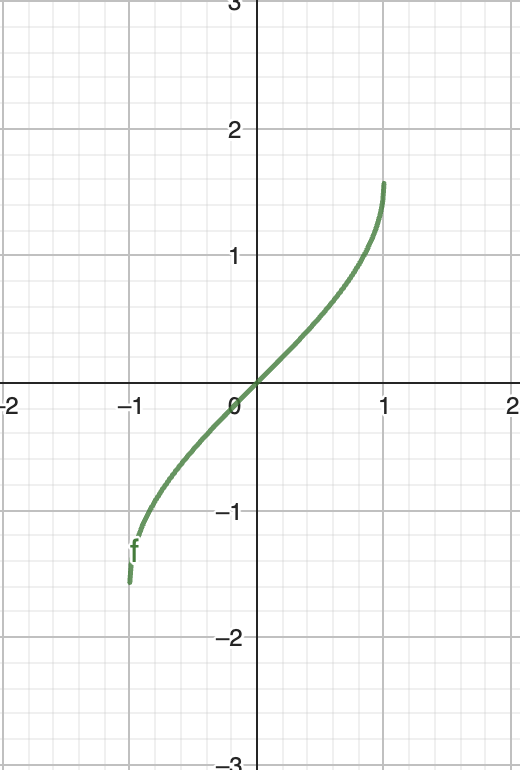
\includegraphics[scale=0.5]{img/tpo1.png}\\
\href{https://github.com/FooolyHARD/Testing-of-Software/blob/36b94ca08662f3774ab9c1f42c43fd15b8e00945/src/main/java/org/senechka/task1/Arcsin.java#L1}{Код функции}\\
Тестовый класс:
\lstinputlisting[language=Python]{src/tpo1.py}
\newpage
\subsection{Задание 2:}
Исходный код алгоритма MergeSort:
\lstinputlisting[language=Python]{src/tpo2_src.py}
\newpage
Один из тестовых классов:
\lstinputlisting[language=Python]{src/tpo2.py}
Учитывая скромность предметной области, имеющейся в варианте, было принято решение дополнить ее своей фантазией:\\
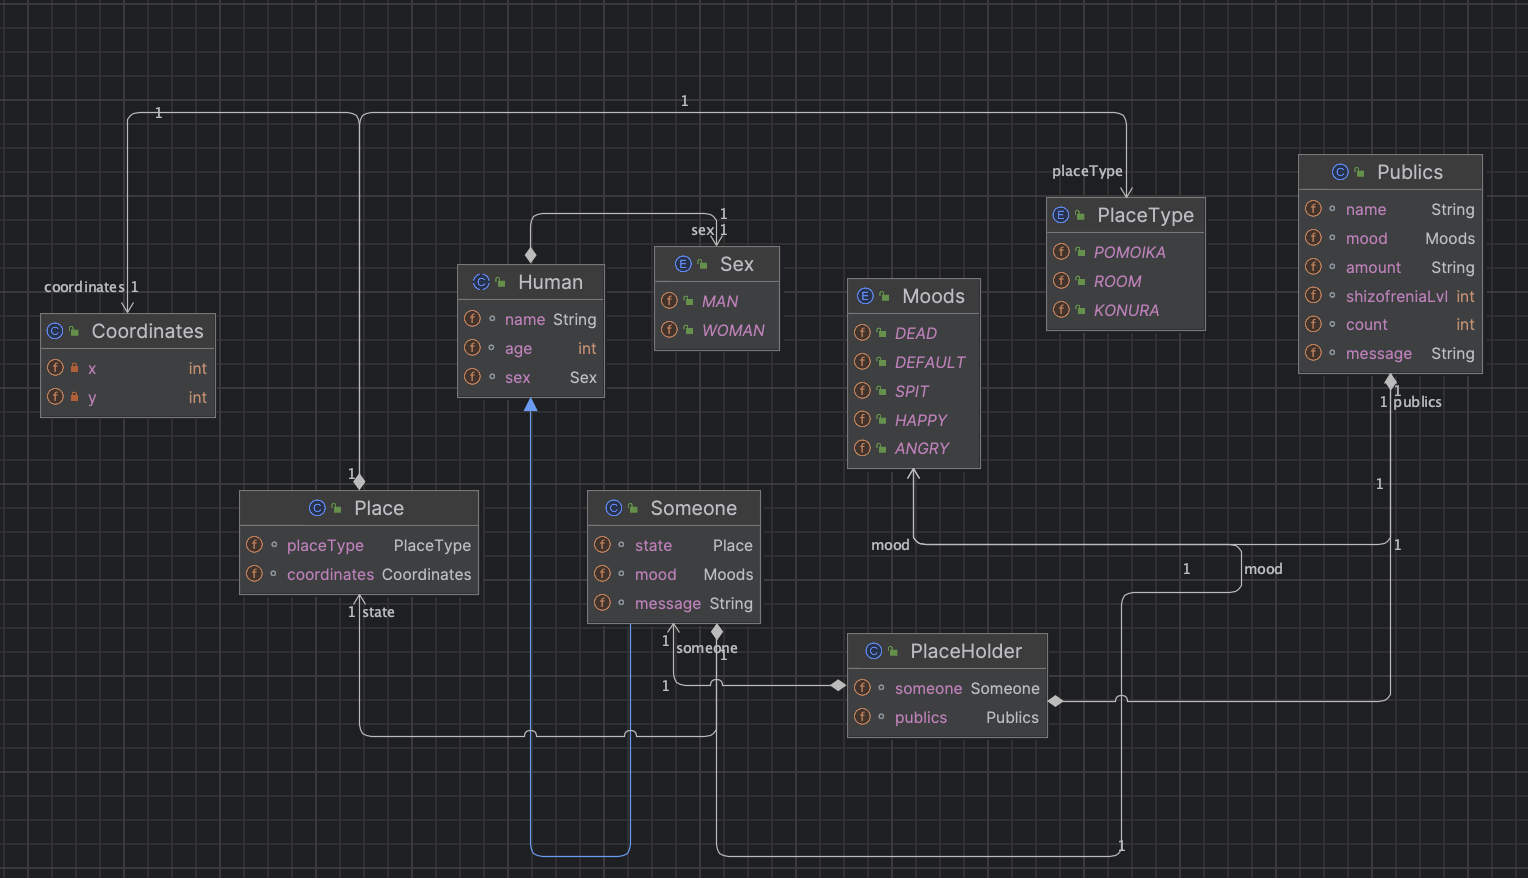
\includegraphics[scale=0.4]{img/tpo3.png}\\
{Пример тестового класса}
\lstinputlisting[language=Python]{src/tpo3.py}
\href{https://github.com/FooolyHARD/Testing-of-Software/blob/36b94ca08662f3774ab9c1f42c43fd15b8e00945/src/main/java/org/senechka/task3}{Код модели}\\
\section{Исходный код}
\hypertarget{p3}{Можно} найти по ссылке \href{https://github.com/FooolyHARD/Testing-of-Software}{на Github}
\section{Вывод}
\hypertarget{p4}{Выполняя} первую лабараторную работу по дисциплине тестирование программного обеспечения я науичлся использовать библиотеку junit и обучился основам работы с тестами в Java.

